\documentclass[letterpaper, 12pt, notitlepage]{report}
\usepackage[plainpages=false, colorlinks, urlcolor=black, citecolor=black,
	linkcolor=blue]{hyperref}
\usepackage{graphicx}

%A LaTeX package which provides macros for the graphical
%representation of the keys on a computer keyboard.
\usepackage{keystroke}

%http://ctan.dcc.uchile.cl/help/Catalogue/entries/floatrow.html
%\usepackage{floatrow}
\usepackage{natbib}
\usepackage{longtable}
\usepackage{epstopdf}
\usepackage[utf8]{inputenc}
\usepackage{txfonts}
\usepackage{listings}
\usepackage{multirow}
\usepackage[polutonikogreek,english,spanish]{babel}
\usepackage{epsfig}
\usepackage{sty/utfsm_tesis}

%Include Table of Contents as the first entry in TOC
\usepackage{sty/xtocinc}

%\usepackage[dvips]{epsfig}
%\usepackage{psfig}

\usepackage{caption}
\usepackage{subcaption}

%% Margenes segun Normas
%% Ancho Legal 21,59cm /  8,5in
%% Alto  Legal 33,02cm / 13,0in
%\paperheight    27.81cm % alto letter
%\paperwidth     21.59cm % ancho
%\hoffset        -1.0in % Seteo a 0 el margen izquierdo
%\voffset        -1.0in % Seteo a 0 el margen superior
%\oddsidemargin  3.80cm % Margen izquierdo (pag. impar)
%% \evensidemargin 2.55cm % Margen izquierdo (pag. par) Acrobat Winkk
%\evensidemargin 2.59cm % Margen izquierdo (pag. par)
%\topmargin      1.00cm % Margen superior
%\headheight     5.00mm % Ancho encabezado
%\headsep        8.00mm % Separacion encabezado-cuerpo
%\textheight     23.5cm % Alto cuerpo
%\textwidth      15.2cm % Ancho cuerpo
%\footskip       1.30cm % Separacion piepag-cuerpo
\parindent      0em
\parskip        2ex

% Fuzz -------------------------------------------------------------------
\hfuzz2pt

% \oddsidemargin	 0cm	% Ancho Legal 21,59cm
% \evensidemargin 0.5cm	% Alto	Legal 35,56cm
% \textwidth	 16.5cm
% \topmargin	  -1.5cm
% \textheight	 22cm

\newlength{\defbaselineskip}
\setlength{\defbaselineskip}{\baselineskip}

\newcommand{\setlinespacing}[1]%
	   {\setlength{\baselineskip}{#1 \defbaselineskip}}
\newcommand{\doublespacing}{\setlength{\baselineskip}%
			   {1.3 \defbaselineskip}}
\newcommand{\singlespacing}{\setlength{\baselineskip}{\defbaselineskip}}

\lstloadlanguages{C++, sh, IDL, make}
\lstset{basicstyle=\small\sffamily, commentstyle=\slshape,
        numbers=left, numberstyle=\tiny, numbersep=10pt,
        extendedchars, frame=lines,
        floatplacement=ht, captionpos=b,
        defaultdialect=[CORBA]IDL}



%descomentar para poner fecha distinta a fecha de compilacion
%\copyrightyear{2015} \submitdate{Mes A\~{n}o}
%\convocation{Mes}{A\~{n}o}

\title{Sistema Recomendador Basado en Confianza para Centros Culturales en la Región Metropolitana}
\author{Sebastián Vidal}

\begin{document}

\selectlanguage{spanish}

\profguia{Hernán Astudillo}
\profcorr{Pablo Cruz}

% Archivo de Agradecimientos
\ack{include/acknowledgements}

% Incluir Resumen
\resumenesp{include/resumen}

% Incluir Abstract
\resumening{include/abstract}

% Incluir Abreviaciones
\abreviaciones{include/glossary}

\beforepreface
\afterpreface

%\numberwithin{equation}{chapter}

% Incluir introduccion
\addcontentsline{toc}{chapter}{Introducci\'on}
\chapter*{Introducci\'on}


\section{Contexto}

Desde su creación en el año 1989, la World Wide Web (www, o W3) ha cambiado las telecomunicaciones permanentemente y ha permitido el intercambio de información entre personas de todo el mundo. Actualmente, la colaboración, interacción e intercambio de información son la fuerza que mueve las aplicaciones web de hoy en día (A esto se le conoce como Web 2.0).  Ejemplos de esto son los blogs, redes sociales, wikis y sitios específicamente desarrollados para compartir contenido creado por usuarios, tales como YouTube\footnote{http://www.youtube.com/} Wikipedia\footnote{http://es.wikipedia.org/} ,  Yelp \footnote{http://www.yelp.com/} o  TripAdvisor\footnote{http://www.tripadvisor.com/}. 
Durante la segunda mitad de la década de los años 2000 hasta ahora se ha mantenido esta tendencia hacia el usuario como la principal fuente de generación de contenido, lo cual se conoce como \" Crowdsourcing \". En el caso de TripAdvisor, el crowsourcing ha significado una plataforma con una cantidad enorme de reseñas y opiniones de usuarios en todo el mundo. Wikipedia, por su parte, ha utilizado el crowsourcing para crear la enciclopedia más grande y completa de todos los tiempos, con más de 5 millones de artículos (CITA) , en su versión en inglés.  El mayor valor de este paradigma ha dado acceso a información que habría sido imposible de generar con el modelo Web 1.0 en el que creador y consumidor eran personas distintas. 

%inicio desarrollo
%archivo definicion del problema
\chapter{Definici\'on del Problema}

Actualmente, la colaboración, interacción e intercambio de información son la fuerza que mueve las aplicaciones web de hoy en día (A esto se le conoce como Web 2.0).  Ejemplos de esto son los blogs, redes sociales, wikis y sitios específicamente desarrollados para compartir contenido creado por usuarios, tales como Youtube, Deviantart ,  Twitch o Newgrounds. 
Con el auge de los dispositivos móviles se ha mantenido esta tendencia a
Ya que ahora, en gran volumen, los usuarios cumplen roles de consumidores y creadores, se hace necesario un mecanismo que permita diferenciar a los usuarios y el contenido que producen, para facilitar el enlace entre un usuario y el contenido que éste desea.
Con esta motivación, nace el área de sistemas de recomendación basados en confianza, sustentados en áreas más antiguas, como los sistemas de recomendación y reputación.
Ya que cualquier persona puede decir cualquier cosa sobre cualquier cosa, uno de los problemas que se presentan, tanto para un usuario común, como para los sitios web, es que dado el alto volumen de información generada, es difícil determinar su nivel de veracidad (ni las intenciones del usuario que las genera).

%archivo estado del arte
\chapter{Estado del Arte}

\section{Estado del Arte}
La colaboración y la interacción entre usuarios de la web han sido claves para el cambio de paradigma que ocurrió para el uso de Internet a principios del siglo XXI, después del estallido de la burbuja “punto com” a finales del año 2001. Hasta ese entonces, el uso de Internet consistía en navegación de los contenidos de una página web estática,  para luego pasar a la siguiente.  El paradigma cambia, de sólo lectura a lectura y escritura, de compañías a comunidades y de portales a plataformas web.\cite{Aghaei2012}

Entre los sitios que sobrevivieron a la crisis están gigantes como Amazon, Google e eBay. Lo que estas empresas tienen en común es que motivaron una participación activa de sus usuarios, generando un ciclo de retroalimentación que aumentó el número de usuarios,  

Con el tiempo, dado el alto volumen de información generada, surgen varios problemas que impiden un uso óptimo de los recursos que ofrece la web. Entre ellos, se pueden encontrar los siguientes, que serán el énfasis en esta memoria.

\begin{itemize}
\item{En plataformas web, un usuario puede ser abrumado por el exceso de contenidos. }
\item{Las fuentes de información son numerosas y, muchas veces, contradictorias. }
\end{itemize}

En respuesta a estas necesidades, existen sistemas capaces de navegar por el contenido de una plataforma web y hacer recomendaciones de ítems a un usuario,  segun los datos disponibles de éste. Además se han desarrollado modelos que describen la confianza entre usuarios de un plataforma, con el objetivo de discriminar entre las diversas fuentes y determinar la más creíble para una persona en particular. 

A continuación se detallarán las implementaciones de ambas soluciones y las formas en que ambas pueden enriquecerse mutuamente.

\subsection{Computación Basada en Confianza}

La confianza es un fenómeno social que se da comúnmente en una comunidad de personas, segun \citep{Marsh1994}, se dice que el ser humano no podria enfrentar las complejidades del mundo sin recurrir a la confianza, ya que es con confianza que somo capaces de razonar de forma sensata a los eventos de la vida diaria. Por ejemplo, cada día salimos de nuestros hogares \textit{confiando} en que seremos capaces de volver y \textit{confiando} en que no tendremos un accidente que nos lleve al hospital. 


En términos generales, existen varias definiciones del concepto de "confianza",  según Morton Deutsch en 1962  el comportamiento de confianza ocurre cuando un individuo percibe un camino ambiguo, el resultado de cual puede ser beneficioso o dañino, y la ocurrencia de un resultado "bueno" o "malo" depende de las acciones de otra persona. Si el individuo elige ir en ese camino, se puede decir que actuó de manera confiada, de lo contrario es desconfiado. Esta definición obedece a la noción de que la estructura básica de la confianza consiste en una decisión.

Otra definición de "confianza", por Gambetta sugiere que "…confianza, (o simétricamente, desconfianza) es un nivel particular de probabilidad subjetiva de que un agente realice una acción en particular, antes de que pueda monitorear dicha acción y en una situación que afecte su propia acción" \citep{Medic2012} . En esta defición es importante aclarar que la probabilidad subjetiva es aquella en que un evento es asignado por el individuo basandose en la evidencia disponible (el individuo asigna la probabilidad en base a su experiencia).

Por último, otra definición que se rescata en la literatura está en \cite{Robillard2010}, la cual es como sigue "La confianza es un estado psicológico que involucra expectativas sobre la competencia, benevolencia, integridad y predictibilidad de otra persona y su voluntad de actuar en base a esas expectativas. Los problemas de confianza surgen en contextos que involucran riesgo, vulnerabilidad, incertidumbre e interdependencia. Las expectativas de confianza se crean principalmente por interacciones de las cualidades percibidas de en quien se confía y factores contextuales que entran en juego cuando se hacen decisiones de confianza".

Lo  que se puede destacar de éstas definiciones es la naturaleza de la confianza, que consiste en la toma de decisiones en contextos de incertidumbre y riesgo, basado en valores arbitrarios. Y es una manera en que comprender y adaptarse a las complejidades del medio en que nos desenvolvemos. Siguiendo con \citep{Marsh1994}, se desataca que la confianza es lo que juega un rol importante en la formación de grupos, su estructura y los comportamientos que se dan dentro de éstos. 

En general se identifican tres tipos de confianza, disposicional, impersonal e interpersonal. 

\begin{itemize}
\item{La confianza disposicional se refiere a un estado interno del individuo, que está dispuesto a confiar. Esta confianza es abierta e independiente de factores externos u otro contexto. Este tipo de confianza se puede subdividir en dos tipos, el tipo A se refere a la creencia del "confiador" en la benevolencia del otro, mientras que el tipo B es la "disposición que, independiente de la benevolencia del otro, se puede obtener un resultado más positivo actuando \textit{como si} se confiase en el otro. \cite{Marsh1994}}



\item{La confianza interpersonal se refiere a aquella en propiedades percibidas o fe en el sistema o institución donde existe la confianza. Un ejemplo de esto es el sistema monetario \cite{Medic2012}.}

\item{Finalmente, la confianza interpersonal se refiere a la que tiene una persona sobre otra directamente, ésto se puede ver también como una confianza disposicional hacia un sistema viviente. Este tipo de confianza depende del contexto y del individuo. Una persona A puede confiar en una persona B para que arregle su computador, pero no para consejos emocionales.}
\end{itemize}
Como se mencionó anteriormente, la confianza no es una propiedad objetiva, sino un grado subjetivo de creencia en una persona, proceso u objeto. El grado puede variar desde confianza ciega a completa desconfianza, o incluso se puede no tener una opinión sobre el nivel de confianza en otra persona (por falta de información). Este nivel es variable en el tiempo, ya que la confianza en otra persona puede aumentar o disminuir según las experiencias que hayamos tenido con ésta. 

Otro aspecto importante de la confianza es que puede aumentar y reforzarse con el uso y disminuir con el desuso, esto se relaciona con la forma en que se razona el proceso de búsqueda de evidencias  para confiar o desconfiar, siendo los datos más recientes los más vigentes y confiables.  \cite{Medic2012}

En el campo de la informática, se conoce al modelamiento de la confianza entre personas como Trust-Based Computing\footnote{ Computación Basada en Confianza, del inglés} \cite{Victor}.
En la literatura \cite{Medic2012,Victor,Artz2007} se menciona que uno de los modelos más antiguos de confianza fue propuesto en el año 1994, por Stephen Paul Marsh, de la Universidad de Strirling [CITA]. Este modelo está establecido sólo con interacciones directas en el proceso de confianza. 

Se separa la confianza en tres aspectos distintos, el básico, general y situacional. 

\begin{itemize}
\item{La confianza básica modela la confianza disposicional, mencionada anteriormente. Se calcula a partir de todas las experiencias acumuladas del agente. Es decir que experiencias buenas llevan a mayor confianza y viceversa. Se usa la notación $T_x^t$ para denotar la disposición de un agente x en un momento t}
\item{La confianza general es la que tiene un agente sobre otro, sin tomar en cuenta alguna situación en específico. Representa simplemente la confianza general en otro agente. Se denota $T_x(y)^t$, la confianza general de un agente $x$ sobre un agente $y$ en un tiempo t }

\item{La confianza situacional es la que un agente tiene sobre otro teniendo en cuenta una situación específica. Se calcula considerando la utilidad de la situación, su importancia y la confianza \textit{general}}

\end{itemize}

Sin embargo, este modelo tenía algunas limitaciones \cite{Medic2012}

En primer lugar, consideraba a la persona en quien se confia como una entidad pasiva. Toda acción es de parte de el \textit{confiador}. Es él o ella quien toma la decisión confiar, después de una serie de cálculos y otros factores . Sin embargo, en el mundo real, la persona a confiar nunca es pasiva, ya que envía señales constantemente al confiador, tanto positivas como negativas. 

La otra limitación que tenía este modelo consiste en que no se captura el rol de la situación en que se confia. En \citep{Medic2012} se explica esto con un ejemplo. Una persona A considera entrar a un taxi de B, quien viene saliendo de un bar. Si B ha llevado a A de forma segura en el pasado numerosas veces antes, y B no muestra señales de estar borracho.¿Confiaría A en B de la misma forma? Lo más probable es que no, incluso aunque B cumpla todos los criterios que exige el modelo.

Tampoco toma en cuenta el rol importante que juega la comunicación en la determinación de confianza.

 Los modelos de confianza que se utilizan actualmente son varios y se pueden clasificar de muchas formas. Una de ellas está descrita en \cite{Victor}, donde se ordenan los modelos según su acercamiento, que puede ser probabilístico o gradual. 

\begin{itemize}
\item{Los modelos probabilísticos operan a un nivel "todo o nada", un agente o fuente puede ser confiable \textit{o no}. Muchas veces se basa este tipo de confianza en el número de transaccones positivas o negativas. Estos modelos se utilizan en redes P2P.}
\item{Un modelo gradual hace una estimación de valores de confianza, cuando el resultado de una acción puede ser positiva hasta cierto nivel, en vez de ser \textit{bueno} o \textit{malo}. Esto representa mejor la forma en que los seres humanos interpretan la confianza. Una persona no opera en términos de \textit{confío} o \textit{desconfío}, sino mas bien se confía \textit{mucho},  \textit{mas o menos} o en otros términos más ambiguos. Estos son los modelos que se utilizan en sistemas de recomendación.}
\end{itemize}

La mayoría de los modelos de confianza ignora completamente la \textit{desconfianza}, o la considera como el final de una misma escala. En \cite{Victor} se propone un modelo que usa una dupla $(t,d)$ con un grado $t$ de confianza y $d$ de desconfianza. Para obtener el valor final de confianza se le resta $d$ a $t$. 

En redes de confianza que existen en la web, lo que ocurre la mayoría de las veces es que para un usuario específico, el resto de los usuarios son desconocidos. Sin embargo hay casos en es útil saber si se puede confiar en un desconocido, y en ese caso, en qué grado es esto posible. Por ejemplo, un usuario desea comprar un producto en un sitio como Amazon, pero se da cuenta de que el producto está mal calificado por otros usuarios. ¿ Son estos comentarios dignos de confianza o no?. 

Existen métricas de confianza \cite{Victor} que calculan un estimado de cuánto confiaría un usuario en otro, basado en relaciones de confianza existentes entre otros usuarios en la misma red. Estas métricas usualmente incorporan técnicas basadas en la suposición de que la confianza es, de alguna manera, transitiva. A estas técnicas se les llama \textit{estrategias de propagación}.

En la figura siguiente es posible ver un ejemplo:

\begin{figure}[hbtp]
\centering
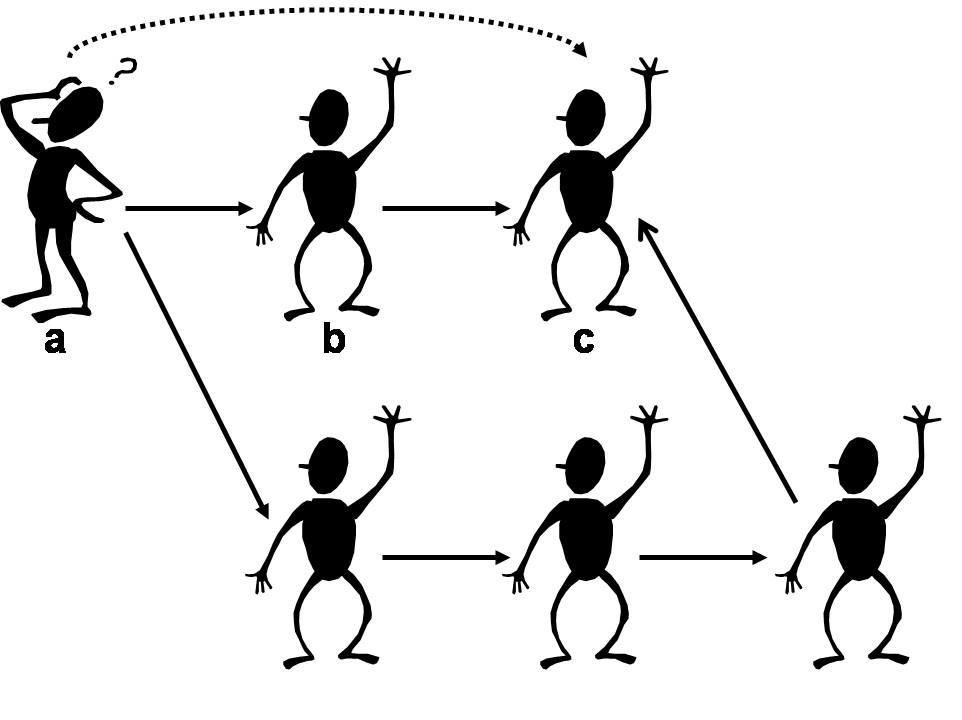
\includegraphics[scale=0.3]{images/trustprop.png}
\caption{Una persona $a$ evalúa si confiar o no en una persona $c$}
\end{figure}

Si una persona $a$ desea saber si confiar en $c$ y sabe que $b$ confía en $c$, se puede decir que $a$ tiene al menos cierto grado de confianza en $c$, por transitividad. 
La estrategia mas básica de propagación se conoce como propagación atómica directa. Este es un modelo que no tiene en cuenta el contexto donde se da la relación de confianza y además usa relaciones transitivas asumiendo que todas las confianzas interpersonales son iguales. 

En modelos probabilísticos de confianza, la forma de propagarse es mediante la multiplicación simple, el cual también se use en técnicas graduales, sin embargo éstas poseen un espectro mas amplio de operadores de propagación. 

En \cite{Victor} se entrega un ejemplo de propagación de confianza:

Suponer el uso de duplas $(t,d)$ con valores de confianza y desconfianza entre 0 y 1, denotando la gradualidad de los atributos y también permitiendo expresar falta de información como un 0. 

\begin{itemize}
\item{$(t_1,d_1)$ es la confianza que tiene el usuario $a$ sobre el usuario $b$}
\item{$(t_2,d_2)$ es la confianza que tiene el usuario $b$ sobre el usuario $c$}
\end{itemize}

Se puede calcular la confianza de $a$ en $c$ como:

\begin{equation}
(t_3,d_3) = (t_1 * t_2, t_1*d_2)
\end{equation}

Esta estrategia de propagación refleja la actitud de valorar información de fuente confiables y descartar información de personas desconocidas.

Alternativamente, se puede calcular la confianza como: 

\begin{equation}
(t_3,d_3) = (t_1*t_2+d_1*d_2-t_1*t_2*d_1*d_2,t_1*d_2+d_1*t_2-t_1*d_2*d_1*t_2)
\end{equation}

Esta estrategia hace asume que una fuente desconfiada está dando información errónea maliciosamente. Por lo tanto $a$ confiará en $c$ si es que $b$ es confiable. Si desconfía de $b$, $a$ hará lo contrario de lo que $b$ sugiere respecto a $c$. En otras palabras, es como el dicho \textit{El enemigo de mi enemigo es mi amigo.}

Estos ejemplos muestran diferencias entre los autores de la literatura en cuanto al valor que se le da a una fuente confiable y qué hacer ante un agente que no se vea confiable.

Una métrica de confianza también debe incluir estrategias de sumatorias, ya que en una red lo suficientemente grande siempre habrá más de un camino desde $a$ hasta $c$.

En estos casos, se pueden utilizar operadores de grafos, tales como camino mínimo, máximo, media aritmética, o promedio ponderado. 

\begin{figure}[hbtp]
\centering
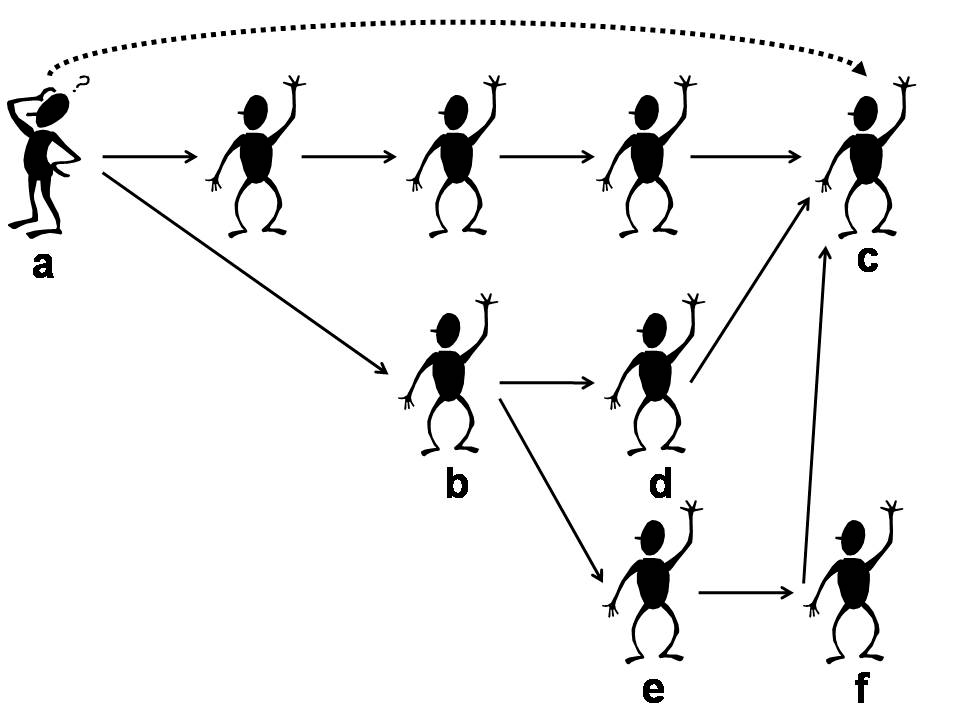
\includegraphics[scale=0.3]{images/trustaggr.png}
\caption{Varios caminos para llegar desde $a$ hasta $c$}
\end{figure}

Los operadores ponderados ofrecen la posibilidad de discriminar caminos y seleccionar aquellos que sean de mayor importancia, lo que entrega mayor flexibilidad para el diseño de una red de confianza. 

Las estrategias de propagación y sumatorias se pueden combinar de distintas formas, obteniendo distintos resultados, según la importancia que se les de a los caminos y arcos del grafo. Incluso el resultado es distinto si se hace una sumatoria antes de la propagación, para primero elegir un camino entre $a$ y $c$ y no tener que consultar los valores de confianzas de cada nodo (Que puede llegar a ser altamente costoso con una red lo suficientemente grande), o incluso por razones de seguridad, evitando exponer los grados de confianza,desconfianza de cada nodo. 

\subsection{Sistemas de Recomendación}

El sistema de recomendación es el segundo pilar sobre el que se sostiene el sistema que se propone para esta memoria.

Un sistema de recomendación es aquel que intenta predecir una respuesta del usuario hacia opciones.

Los sistemas de recomendación se pueden agrupar en varias categorías, sin embargo las más comunes son \cite{Resnick1997,Girgin}

\begin{itemize}
\item{Sistemas basados en contenidos. Son aquellos que examinan las propiedades del ítem recomendado. Por ejemplo, si un usuario de Netflix mira muchas películas del género \textit{terror}, entonces el sistema le recomendará una película de terror}

\item{Filtrado Colaborativo. Son sistemas que recomiendan ítems basado en la similitud entre usuarios y/o ítems. Los ítems recomendados a un usuario son los que prefieren usuarios similares}
\end{itemize}

En un sistema recomendador, se pueden identificar dos clases de entidades, \textit{usuarios} e \textit{ítems}[CITA]. Los datos en s[i se representan en una \textit{Matriz de Utilidad}, que da a cada dupla usuario-item un valor que representa el grado de preferencia (Algo así como las \textit{estrellas} en diversos sitios que permiten clasificar películas) con números que van desde el 1 al 5. Se asume que la matriz no estará llena, por lo que la mayoría de las entradas estará en estado desconocido (No hay información sobre la preferencia del ítem).

\begin{figure}
\centering
\begin{tabular}{l*{6}{c}r}
                  & Rapido y Furioso & Los 33 & Capitán América & Intensa-Mente & Los Vengadores  & 50 Sombras de Grey  \\
\hline
A          &  &  & 1 & 5 & 1 & 5   \\
B          &  & 2 & 5 &  & 4  & 1   \\
C              & 1 &  &  & 2 & 5  &1   \\
D       & 5 & 2 &  &  &   & 3   \\
E		 & 2 & 2 & 2 & 2 & 2  & 2   \\

\end{tabular}
\caption{Las estrellas que dan los usuarios A, B, C y D a distintas películas}
\end{figure}

Teniendo la matriz, el objetivo ahora es predecir los puntajes que habrá en los espacios en blanco. Por ejemplo, el usuario C no ha visto Capitán América, pero tiene gustos similares al usuario A, ya que ambos vieron una película del mismo género (Los Vengadores) y ambos expresaron preferencia por dicha película, sería razonable asumir que al usuario C probablemente le gustaría ver Capitán América.

Es importante notar que no es necesario llenar todos los vacíos en esta matriz, basta con llenar los que vayan a tener los ratings más altos.

Ya que una de las bases de un sistema de recomendación es encontrar usuarios similares entre sí, hay que mencionar las formas en que se puede medir la similaridad de dos individuos.

Una de las formas consiste en determinar el índice Jaccard entre usuarios, siguiendo con la matriz del ejemplo,  tomando las preferencias que tiene cada usuario con las películas como si fueran conjuntos de muestreo. 

El índice se calcula como:

\begin{equation}
I_j = \cap / \cup
\end{equation}

Donde $\cap$ es la intersección entre los conjuntos (los elementos que tienen en común) y $\cup$ es la unión entre los conjuntos (la suma de todos los elementos que están en los dos conjuntos). Esta técnica ignora el puntaje que asigna cada usuario a cada película y sólo se preocupa de las películas que ambos hayan visto.

Dicho esto, revisando los ejemplos, comparando los usuarios C y D, se puede ver que su unión es 5 y su intersección es 1. Por lo tanto $1 / 5 = 0,2$, su índice Jaccard es bajo y efectivamente, es porque sólo han visto una película en común. 

Un caso de similaridad es de B y C, que tienen un índice Jaccard de $3/6 = 0,5 $.

Una forma de tener en cuenta las preferencias de los usuarios a la hora de determinar si son similares o puede ser redondeando los valores hacia 0 o 1, como intentando aproximar si a la persona le gustó o no la película. Si se reemplazan los ratings de 3, 4 y 5 estrellas por un 1, se dice que al usuario le gustó la película (Siendo optimistas y asumiendo que el valor medio, 3, también dice que a la persona le gustó la película). De lo contrario, se cambia el rating por un 0.

\begin{figure}[h!]

\begin{tabular}{l*{6}{c}r}
                  & Rapido y Furioso & Los 33 & Capitán América & Intensa-Mente & Los Vengadores  & 50 Sombras de Grey  \\
\hline
A          &  &  & 0 & 1 & 0 & 1   \\
B          &  & 0 & 1 &  & 1  & 0   \\
C              & 0 &  &  & 0 & 1  &   \\
D       & 1 & 0 &  &  &   & 1   \\
E 		& 0 & 0 & 0 &  0&  0 & 0   \\

\end{tabular}
\caption{Se cambiaron los 3,4 y 5 por 1, y los 1 y 2 por 0}
\end{figure}

Ahora el índice Jaccard para C y D es $0 / 3 = 0$ y para B y C es $ 1 / 2 = 0,5$.

Por último es posible utilizar la correlación de Pearson \cite{Girgin,Victor}. Lo primero es normalizar los valores, restándoles a cada uno su promedio. Así, se convierten bajos ratings en números negativos y altos en positivos. 

\begin{figure}[h!]

\begin{tabular}{l*{6}{c}r}
                  & Rapido y Furioso & Los 33 & Capitán América & Intensa-Mente & Los Vengadores  & 50 Sombras de Grey  \\
\hline
A          &  &  & -1 & 3 & -1 & 3   \\
B          &   &  & 3 & 0 &  2 & -1   \\
C              & -0.5 & -1.5 &-1.5  & 0.5 & 3.5  &  -0.5  \\
D       & 1 & 0 &  &  &   & 1   \\
E 		& 0 & 0 & 0 &  0&  0 & 0   \\

\end{tabular}
\caption{La matriz de ejemplo con valores normalizados}
\end{figure} 

Luego se calcula la similaridad como el seno del ángulo entre los vectores que representan a cada usuario. Por ejemplo, para calcular la similaridad entre el usuario B y el C se hace el siguiente cálculo:

\begin{equation}
\frac{3*-1.5 + 2*3.5+-1*-0.5}{\sqrt{3^2+2^2+(-1)^2}*\sqrt{(-0.5)^2+(-1.5)^2+(-1,5)^2+o.5^2+3,5^2+(-0.5)^2}}  = 0.3785
\end{equation}

Esta técnica de filtrado colaborativo toma en cuenta las películas que ambas personas vieron y los ratings que entregan a cada una.

Cuando ya se tiene la correlación entre dos personas, se puede predecir la preferencia de un usuario $u$ por un ítem $i$ con la siguiente fórmula, según \cite{Girgin}

\begin{equation}
pred(u,i) = \overline{r} + \frac{\sum\limits_{vecindario} Sim(u,n) * (r_ni - \overline{r_n} )}{\sum\limits_{vecindario} Sim(u,n)}
\end{equation}

Donde $Sim(u,n)$ es la similitud entre el usuario $u$ y el usuario $n$, $\overline{r}$ es el rating promedio (de todos los usuarios) , $r_ni$ es el rating que da el usuario $n$ al ítem $i$ y $\overline{r_n}$ es el rating promedio que entregó el usuario $n$.  

\subsection{Mejorando un Sistema de Recomendación con una Red de Confianza}

Según [CITA], a pesar de recibir mejoras significativas, los sistemas de recomendación siguen teniendo problemas importantes, en especial los de filtrado colaborativo. 



Lo que ocurre es que los usuarios generalmente entregan ratings de una fracción minúscula de los ítems disponibles, por lo tanto, los algoritmos tienen problemas para hallar buenos vecindarios y la calidad de las recomendaciones puede sufrir a causa de esto. 

También es difícil generar recomendaciones para usuarios nuevos en un sistema (usuarios que partan en frío en una plataforma),  ya que no han calificado un número suficiente de ítems y por lo tanto es difícil encontrar usuarios similares.

Ya que los sistemas de recomendación se utilizan en sitios de comercio es frecuente que usuarios mal intencionados abusen del sistema de calificaciones para intentar mejorar el posicionamiento de un producto en el algoritmo de recomendación.

Por último, \cite{Victor} sostiene que las personas tienden a confiar más en recomendaciones hechas por personas de confianza más que por usuarios anónimos similares. Por lo tanto se justifica el uso de redes de confianza para mejorar un sistema de recomendaciones.

En la vida real, una persona que quiera evitar un mal negocio consulta primero a un amigo y si dicho amigo no sabe, él consulta a un amigo suyo, así sucesivamente, hasta que alguien que aparezca alguien que conozca sobre el tema (un recomendador).  

\begin{figure}[hbtp]
\centering
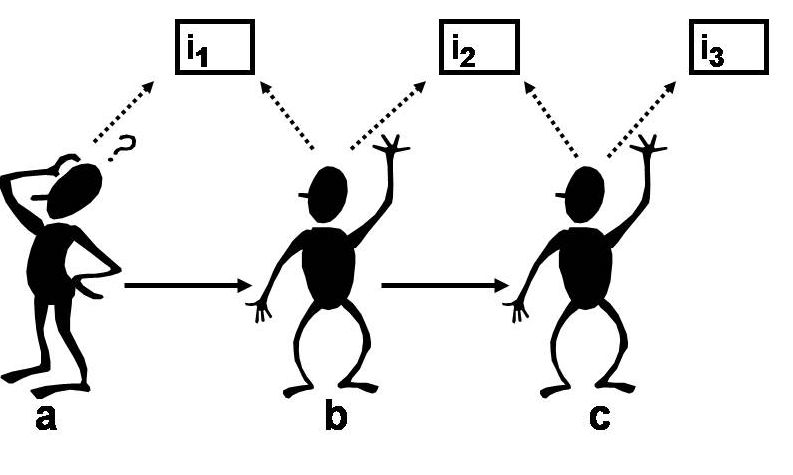
\includegraphics[scale=0.3]{images/trustrec.png}
\caption{Relaciones de confianza en sistemas recomendadores}
\end{figure}

En la figura 6 se describe una situación donde la líneas sólidas denotan la relación de confianza entre usuarios. En un escenario sin una red de confianza, un filtrador colaborativo no podrías generar una predicción para el ítem $i_3$ para el usuario $a$, por falta de información. Pero usando las relaciones de confianza se puede usar una estrategia de propagación que relacione la confianza de $a$ en $c$ y según eso predecir el rating que el usuario $a$ daría al ítem $i_3$. Por ejemplo, si el usuario $a$ confía en $c$ (por transitividad) y al usuario $c$ le gusta el ítem $i_3$, entonces se podría decir que probablemente al usuario $a$ también le guste dicho ítem.

Además de resolver el problema de escasez de información, este acercamiento también puede aliviar el problema con usuarios que comiencen en frío en la plataforma. 

También, al usar redes de confianza que apoye al sistema de recomendación se puede minimizar el efecto de usuarios malintencionados.

Los sistemas de recomendaciones basados en confianza en dos categorías, según la forma en que se obtienen los valores de confianza \cite{Victor}

\begin{itemize}
\item{Sistemas que obtienen los valores de confianza directamente desde inputs de usuarios}
\item{Sistemas que infieren valores de confianza, basándose en el historial de un usuario o en reglas de transitividad de usuario a usuario}
\end{itemize}

Los sistemas que obtienen la información de confianza directamente usan estos valores para determinar cuáles opiniones deberían ser ponderadas más o menos, hay distintas formas de hacer esta ponderación.

Anteriormente, en la ecuación (5) se llega a un rating predicho. Si la confianza entre un usuario $a$ y un usuario $b$ se puede expresar como $t_{u,b}$ (Recordar que este valor puede ir entre 0 y 1). Al multiplicar $t_{u,b}$ por el valor predicho $pred(u,i)$, se puede disminuir el rating esperado, si viene de un usuario poco confiable. 

\begin{equation}
pred_conf(u,i) =  \frac{\sum\limits_{vecindario} t_{u,b} *pred(u,i)}{\sum\limits_{vecindario} t_{u,b}}
\end{equation}

En este caso, el vecindario son todos los usuarios que opinaron sobre el ítem $i$.

Volviendo a la ecuación (5), existe un método llamado "Trust-based collaborative filtering" \footnote{Filtrado Colaborativo, basado en confianza.} que consiste en reemplazar la similitud entre usuarios $Sim(u,n)$ por la confianza entre éstos $t_{u,n}$, ya que según [CITA] la confianza y la similaridad están correlacionados. 


\begin{equation}
pred(u,i) = \overline{r} + \frac{\sum\limits_{vecindario} t_{u,n} * (r_ni - \overline{r_n} )}{\sum\limits_{vecindario} t_{u,n}}
\end{equation}

También \cite{Victor} propone limitar el vecindario a usuarios que tengan un nivel de confianza por sobre un mínimo establecido. Esto se conoce como Trust-based filtering.

Existen alternativas también para calcular el valor $t_{u,b}$, una de ellas, conocida como TidalTrust [CITA] consiste en:

\begin{itemize}
\item{Permitir sólo caminos cortos entre el usuario $a$ y el $c$, ya que son los que entregan resultados más precisos [CITA], para ésto se determina un largo variable para el camino y se busca el más corto}
\item{Permitir sólo información que provenga de usuarios con un nivel mínimo de confianza. Éste se determina cómo el valor máximo del peso de un camino (El peso de un camino está determinado por el valor más bajo de confianza)} 
\item{Por lo tanto, el vecindario en la ecuación (5) queda definido como todos aquellos usuarios que superen el mínimo establecido anteriormente}
\end{itemize}

Otra técnica se llama MoleTrust. Es una idea similar a TidalTrust, se diferencia en que obtiene valores de confianza desde todos los caminos que lleven desde el usuario $a$ al usuario $c$, con un largo límite definido $d$. La otra diferencia con TidalTrust es que también se define manualmente el nivel de confianza mínimo a aceptar (En [CITA] se definen valores de confianza aceptables desde 0,6 hasta 1).

El problema con los algoritmos descritos anteriormente es que requieren que los usuarios describan explícitamente el nivel de confianza con otros usuarios. Ésto puede no ser siempre práctico, por lo que existen algoritmos que pueden inferir estimaciones de valores de confianza, sin información explícita, según el comportamiento histórico de cada usuario, una persona que haya dado opiniones valoradas por la comunidad será más confiable para el resto de los usuarios, en general.

Una forma es implementar un sistema de reputación, que \cite{Victor} describe como confianza a nivel de perfil y de ítem. 

Para esto, se genera una predicción $p_{a,i}$ del rating que el usuario  $u$ colocaría sobre el ítem $i$ en el que está interesado el usuario objetivo $a$, si la diferencia está dentro de un rango $\epsilon$ con respecto al rating que el usuario realmente puso, se dice que $u$ acertó.

Así, se calcula la confianza $t^P_{a,u}$ a nivel de perfil desde $a$ hacia $u$ como el porcentaje de veces que el usuario $u$ acertó.

También se puede calcular la confianza a nivel de ítem $t^P_{a,u}$ como el porcentaje de predicciones sobre el ítem $i$ acertadas.

\cite{Victor} Concluye al comparar los sistemas de recomendación con y sin redes de confianza entregan resultados similares, sin embargo, los sistemas sin redes de confianza tienen peor rendimiento en ítems que tienen opiniones muy contradictorias.
%archivo propuesta
\chapter{Propuesta}



%archivo implementacion
\chapter{Implementaci\'on}

Para facilitar la comprensión del funcionamiento del algoritmo, se va a usar el siguiente ejemplo:

\begin{figure}
\centering
\begin{adjustbox}{max width=\textwidth}
\begin{tabular}{l*{6}{c}r}
                  & Plaza de Armas & Cerro Sta. Lucia & Cerro San Cristobal & Museo de Bellas Artes & Quinta Normal  & Teatro Municipal & Centro GAM \\
\hline
Juan          & 5 & 4 & 2 &   & 1 &   &   \\
\hline
Ignacio       & 3 &   & 2 &   & 5 &   & 4 \\
\hline
Perla         & 3 & 3 &   & 1 & 4 & 3 &   \\
\hline
Inés          & 5 & 5 &   & 1 & 2 &   & 5 \\
\hline
Sam          & 1 &  &   &  &  & 4  & 3 \\


\end{tabular}
\end{adjustbox}
\caption{Las estrellas que dan los usuarios A, B, C y D a distintas películas}

%otra screenshot de algún item con todas sus reviews, y con la pantalla para escribir una

\end{figure}

En este ejemplo, el usuario que entra al sistema y cuyos puntajes son predichos se conoce como consumidor, en este caso es el Usuario 1.

Cada ítem para el cual el consumidor aún no ha escrito una review y que se encuentre a cierta distancia geográfica es un potencial ítem recomendado, pero antes es necesario conocer qué puntaje le asignaría el consumidor.

\begin{figure}
\centering
\begin{adjustbox}{max width=\textwidth}
\begin{tabular}{l*{6}{c}r}
                  & Plaza de Armas & Cerro Sta. Lucia & Cerro San Cristobal & Museo de Bellas Artes & Quinta Normal  & Teatro Municipal & Centro GAM \\
\hline
\rowcolor{yellow} Juan          & 5 & 4 & 2 &   & 1 &   &   \\
\hline
Ignacio       & 3 &   & 2 &   & 5 &   & 4 \\
\hline
\rowcolor{yellow}Perla         & 3 & 3 &   & 1 & 4 & 3 &   \\
\hline
\rowcolor{yellow}Inés          & 5 & 5 &   & 1 & 2 &   & 5 \\
Sam          & 1 &  &   &  &  & 4  & 3 \\


\end{tabular}
\end{adjustbox}
\caption{La misma tabla de la figura x, imaginar que se quiere conocer el puntaje que Juan dará al Museo de Bellas Artes, para eso se deben tener en cuenta sólo los usuarios que hayan visitado este lugar, o sea, Perla y Inés.}

\end{figure}

El proceso de calcular el puntaje predicho para cada ítem se conoce como sesión. Como se puede notar, cada ítem candidato implica una sesión de recomendación.

Comenzando por el primer ítem candidato, al iniciar la sesión, el sistema consulta por todas las reviews que hayan sido escritas sobre el ítem actual. Los usuarios que escribieron estas reviews se conocen como productores.

De este grupo de productores, se escogen sólo los que hayan escrito reseñas sobre al menos dos ítems sobre los que el consumidor haya también dado su opinión.
\newcolumntype{g}{>{\columncolor{yellow}}c}
\begin{figure}
\centering
\begin{adjustbox}{max width=\textwidth}
\begin{tabular}{|c|g|g|c|c|g|c|c|}

                  & Plaza de Armas & Cerro Sta. Lucia & Cerro San Cristobal & Museo de Bellas Artes & Quinta Normal  & Teatro Municipal & Centro GAM \\
\hline
Juan          & 5 & 4 & 2 &   & 1 &   &   \\
\hline
\rowcolor{white}Ignacio       & 3 &   & 2 &   & 5 &   & 4 \\
\hline
Perla         & 3 & 3 &   & 1 & 4 & 3 &   \\
\hline
Inés          & 5 & 5 &   & 1 & 2 &   & 5 \\
\hline
Sam          & 1 &  &   &  &  & 4  & 3 \\
\hline

\end{tabular}
\end{adjustbox}
\caption{Tabla x, pero destacando que para el cálculo del puntaje al Museo de Bellas artes, sólo se tomaran en cuenta lugares que hayan sido visitados por los tres usuarios, Juan, Perla e Inés.}

\end{figure}


En la sección de estado del arte se describieron varias formas en que se pueden integrar los algoritmos de recomendación con los de trust. Para este dominio en particular, ya que se intenta hacer un acercamiento al comportamiento observado en la vida diaria entre personas, se decidió que se utilizará el trust como un umbral, en el que la opinión de una persona ''no confiable'' se considera inválida y por lo tanto, es ignorada. 

Por lo tanto, después de determinar los posibles usuarios productores, existe otro filtro que determina quiénes serán de confianza. Después de obtener la lista inicial de productores, se determina el nivel de trust que tiene el consumidor con cada uno de los productores. Si no existe una relación directa de trust entre el consumidor y el posible productor, ésta se calcula mediante ''tidal trust''. Una vez que se tiene el valor de trust, el productor candidato es removido de la lista si es que su trust con el consumidor es menor a 0.5, en caso contrario, permanece en la lista. 

Luego, para estimar numéricamente el parecido de las opiniones del consumidor con cada productor, se utiliza la correlación de Pearsson (cita). La idea detrás de esta lógica es que mientras más parecido sea el consumidor con un productor, más peso tendrá éste sobre la estimación del puntaje predicho. Empezando por Juan y Perla:

\begin{figure}

\begin{equation}
sim(u,n)=\frac{\sum_{i=1}^{n}(u_i-\bar{u})(n_i-\bar{n})}{\sqrt{\sum_{i=1}^{n}(u_i-\bar{u})^2}+\sqrt{\sum_{i=1}^{n}(n_i-\bar{n})^2}}
\end{equation}
\caption{La similitud entre dos conjuntos, según la correlación de Pearsson, en este caso, interpretar los valores de $u$ como las estrellas que ha dado Juan a los lugares que visitó y los de $n$ los que ha dado Perla. }

\end{figure}
Conociendo el puntaje que ha puesto en promedio cada productor, $\bar{u}$ para Juan y $\bar{n}$ para Perla, se calcula la diferencia con el puntaje dado. Reemplazando con los promedios y los valores de reseñas, se tiene:


\begin{equation}
\frac{3*-1.5 + 2*3.5+-1*-0.5}{\sqrt{3^2+2^2+(-1)^2}*\sqrt{(-0.5)^2+(-1.5)^2+(-1,5)^2+o.5^2+3,5^2+(-0.5)^2}}  = 0.3785
\end{equation}


Este proceso se repite para cada dupla de consumidor-productor posible.

Con esto, se tiene el numerador de la ecuación (referencia), el denominador es el producto de las sumatorias de las desviaciones estándares, para Juan y para Perla.

Con esto, se llega finalmente a un puntaje estimado, que dará el consumidor al ítem actual. Este proceso se repite para cada ítem candidato.
Luego, cuando ya se tienen todos los puntajes predichos, se considera como recomendables sólo los ítems cuyo puntaje estimado sea al menos 3 estrellas.


\begin{figure}
\centering
\begin{adjustbox}{max width=\textwidth}
\begin{tabular}{|c|c|c|c|}
\hline
                &   Museo de Bellas Artes & Teatro Municipal & Centro GAM \\

\hline
Puntaje Predicho Juan          & 1.28  &  3.60  & 3.09  \\
\hline


\end{tabular}
\end{adjustbox}
\caption{Se pueden ver los puntajes que el sistema predice para Juan, se puede ver que el sistema estima que a Juan no le va a gustar el Museo de Bellas Artes, sin embargo, se puede ver que dará puntajes por sobre 3 estrellas al Teatro Municipal y al Centro GAM, por lo tanto se les recomienda esos lugares a Juan.}

\end{figure}

% otra vista que muestra la pantalla de recomendación

Son estos los ítems que el sistema va a mostrar en la vista de recomendados, ordenados de mayor a menor puntaje. 

%fin desarrollo

%archivo conclusiones
\chapter*{Conclusiones}
\addcontentsline{toc}{chapter}{Conclusiones}




%\backmatter
%\cleardoublepage

\singlespacing
\cleardoublepage

\bibliographystyle{plain}
\bibliography{bib/papers}

\end{document}
